\subsection{Main comparison on the repaired simulator}\label{sec:main}
Tables~\ref{tab:rev_vs_fp} and~\ref{tab:rev_vs_adam} give the gap of every device--algorithm pairing over five seeds, against
FP-SGD (the same network, learning rate, initialisation and data order with an exact update) and against digital Adam at its
own selected learning rate. Every arm of a seed now shares its initial weights and its data order (checked by hash in every
record). The FP-SGD learning rate is reused for every device arm: this is a restricted question (what happens when the FP-SGD
rate is reused), not a fair-tuning comparison of the algorithms; Section~\ref{sec:scale} tunes each arm separately.

\paragraph{Against FP-SGD.}
\begin{itemize}
\item \textbf{Plain SGD exceeded the line} in \RVSgdPubFail{} of the \RVSgdPubN{} cells of the four published devices, at the
      FP-selected learning rate.
\item \textbf{All three tasks:} \RVAllThreeFpN{} pairings pass on every task: \RVAllThreeFpList. No TTv2 pairing does: with the
      pulse reset, TTv2 fails on CIFAR on every published device.
\item \textbf{Per task,} \RVMnistFpPassN, \RVCifarFpPassN{} and \RVLmFpPassN{} of the \RVMnistFpCellN{} device cells pass on
      MNIST, CIFAR and the LM. W/YSZ/WO$_x$ fails on CIFAR and the LM with every algorithm, and MO-ECRAM fails on the LM.
\item \textbf{Best cells:} \RVMnistFpBestCell{} on MNIST (\RVMnistFpBestGap\,pp), \RVCifarFpBestCell{} on CIFAR
      (\RVCifarFpBestGap\,pp) and \RVLmFpBestCell{} on the LM (\RVLmFpBestGap\,\%). A negative gap whose interval includes zero
      is not evidence of superiority; and because these are the best of many cells, they are optimistic.
\end{itemize}

\paragraph{Against Adam.} Digital Adam is the stronger baseline. On the LM FP-SGD is \RVLmFpSgdVsAdamPct\,\% worse in bits per
byte than Adam, and \textbf{no analog cell comes within the 5\,\% line of Adam}: the best, \RVLmAdamBestCell, is
\RVLmAdamBestGap\,\% worse (\RVLmAdamPassN{} of \RVLmAdamCellN{} cells pass). On MNIST and CIFAR, where Adam and FP-SGD are
close, \RVMnistAdamPassN{} and \RVCifarAdamPassN{} cells pass against Adam. No pairing passes all three tasks against Adam
(\RVAllThreeAdamN). The analog results are therefore close to the FP-SGD comparator on these tasks, not to the best digital
training in this study.

\paragraph{The margins.} The lines are practical non-inferiority margins, not equivalence: on MNIST a 2\,pp loss from
\RVMnistFp\,\% roughly doubles the error rate. UNRESOLVED means insufficient evidence against the margin, never adequate
performance. The mean digital baselines are \RVMnistFp\,\% and \RVMnistAdamMetric\,\% on MNIST, \RVCifarFp\,\% and
\RVCifarAdamMetric\,\% on CIFAR, and \RVLmFp{} and \RVLmAdamMetric{} bits per byte on the LM (FP-SGD and Adam). The FP-SGD seed standard deviation is \RVCifarFpSd\,pp on CIFAR and \RVLmFpSd{} bits per byte on the LM.

\paragraph{What the update loses.} Two properties of the repaired simulator matter for reading these results.
\begin{itemize}
\item \textbf{Clipping.} The TT family drives its $A$ arrays at ten times the SGD rate, which exceeds the $BL=31$ pulse budget
      in the largest layers: the mean lost fraction of the requested $A$ update reaches \RVLostCifarTtLayerMeanMaxPct\,\% in the
      CIFAR output layer and \RVLostLmTtLayerMeanMaxPct\,\% in the LM embedding (plain SGD at most \RVLostLmSgdLayerMeanMaxPct\,\%
      in any layer's mean). These are means over the device runs of one layer; the worst single layer record loses
      \RVLostMaxPct\,\% (\RVLostWorstDev{} \RVLostWorstAlg, \RVLostWorstTask{} output layer). The logged fraction is the
      discarded unsigned expected pulse mass, not the norm of the lost signed gradient after cancellation. Clipping the line
      probabilities at one is the update-management policy chosen here (pulse length and update management are configurable
      choices~\cite{rasch2021aihwkit}), not a property of the devices; it caps the effective $A$ rate in those layers, and the
      aggregate update itself is an approximation (Section~\ref{sec:fidelity}).
\item \textbf{Reset residual.} With at most 62 pulses per weight, the pulse reset leaves a residual on the read $A$
      columns. Averaged with every layer and run weighted equally (a macro-average of the per-layer means), it is
      \RVResetResidMean{} nominal steps; pooled over all reset events it is \RVResetResidPooled{} (Li-ECRAM
      \RVResetResidPooledEcramLiTangTwoZeroOneEight, protonic-inspired \RVResetResidPooledProtonicOnenTwoZeroTwoTwo, MO-ECRAM
      \RVResetResidPooledEcramMoKimTwoZeroOneNine); the largest layer mean is \RVResetResidMax{} (MO-ECRAM). Reset pulses are
      \RVResetShareMean\,\% of all pulses as the mean of the per-run fractions, and \RVResetSharePooled\,\% pooled (all reset
      pulses over all pulses). The macro-averages say what a typical layer and run see; the pooled numbers what the arrays
      receive in total.
\end{itemize}

\paragraph{Ideal-device reference.} The same algorithms on an ideal device (symmetric, constant step, 1000 levels, no noise, no
spread, exact reference) are the rows ``Ideal 1000-level'' of the tables (deviation R2). On MNIST every algorithm passes on it.
On CIFAR and the LM none does: plain SGD loses \RVCifarIdealOneZeroZeroZeroSgdVsFpGap\,pp and
\RVLmIdealOneZeroZeroZeroSgdVsFpGap\,\% (stochastic pulse updates on a 1000-level grid at the FP-SGD rate), and c-TTv2 and AGAD
lose \RVCifarIdealOneZeroZeroZeroCttvTwoVsFpGap{} and \RVCifarIdealOneZeroZeroZeroAgadVsFpGap\,pp on CIFAR, far more than on the
saturating Li-ECRAM and protonic-inspired devices. With the settings selected here, the TT family relies on the device's own
saturation as the decay of its accumulator; the ideal device has none. This is a property of these algorithm settings, not a
general requirement that devices saturate: a sufficiently precise symmetric device can implement SGD, as the MNIST row shows.
This reference keeps stochastic pulse counts, bounds, transfer thresholds and the selected update management, so it is not an
exact-update, algorithm-only TT reference, and its MNIST success does not show that every other failure is an unavoidable
device limitation.

\begin{figure}[!ht]\centering
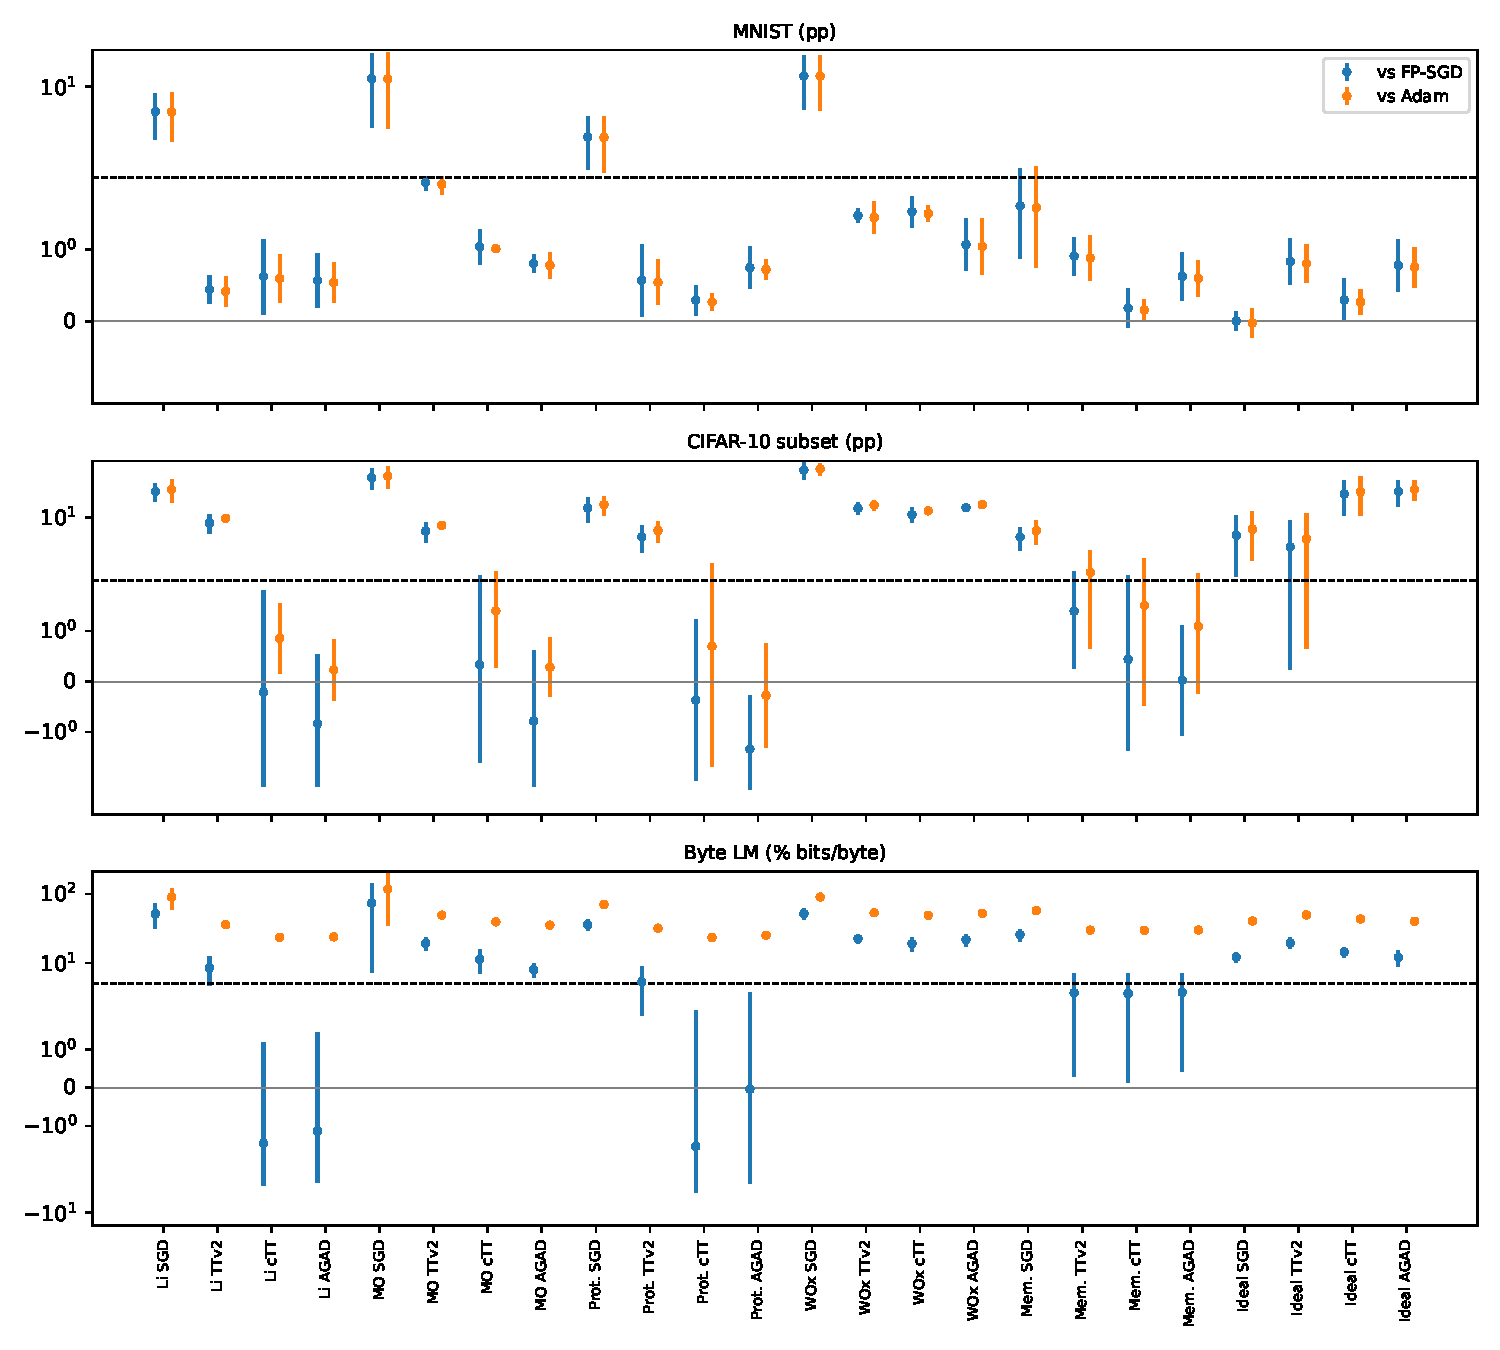
\includegraphics[width=\linewidth]{figs/fig_rev_main}
\caption{Repaired simulator: gap to FP-SGD (blue) and to digital Adam (orange) per device and algorithm, mean and 95\,\% interval
over 5 seed-matched runs (symmetric-log axis); the dashed line is the gap line.}\label{fig:rev_main}
\end{figure}
\begin{table*}[t]\centering\footnotesize\caption{Revised main table (repaired simulator): gap to FP-SGD at the same learning rate, mean [95 \% $t$-interval] over 5 seeds paired by seed (same initialisation and data order); MNIST and CIFAR in accuracy points, LM in \% of bits per byte; P/F/U = PASS/FAIL/UNRESOLVED against the absolute lines 2 pp, 2 pp, 5 \%.}\label{tab:rev_vs_fp}
\begin{tabular}{llccc}\toprule Device & Alg. & MNIST & CIFAR & LM\\\midrule
Li-ECRAM & SGD & 6.41 [3.90, 8.93] F & 19.19 [14.94, 23.44] F & 51.64 [31.63, 71.64] F\\
Li-ECRAM & TTv2 & 0.44 [0.24, 0.64] P & 8.65 [6.64, 10.66] F & 8.51 [4.72, 12.30] U\\
Li-ECRAM & c-TTv2 & 0.62 [0.10, 1.14] P & -0.21 [-2.22, 1.80] P & -1.45 [-4.07, 1.18] P\\
Li-ECRAM & AGAD & 0.57 [0.19, 0.94] P & -0.84 [-2.20, 0.53] P & -1.13 [-3.69, 1.44] P\\
MO-ECRAM & SGD & 11.51 [4.88, 18.14] F & 27.24 [20.15, 34.34] F & 73.84 [7.32, 140.36] F\\
MO-ECRAM & TTv2 & 1.93 [1.82, 2.03] U & 7.04 [5.25, 8.83] F & 19.31 [15.05, 23.57] F\\
MO-ECRAM & c-TTv2 & 1.04 [0.79, 1.28] P & 0.33 [-1.60, 2.27] U & 11.33 [7.11, 15.55] F\\
MO-ECRAM & AGAD & 0.80 [0.67, 0.93] P & -0.79 [-2.19, 0.62] P & 7.98 [6.08, 9.87] F\\
Protonic-inspired & SGD & 4.09 [2.29, 5.88] F & 12.66 [8.83, 16.49] F & 35.99 [29.87, 42.10] F\\
Protonic-inspired & TTv2 & 0.57 [0.07, 1.07] P & 6.08 [4.06, 8.10] F & 5.34 [1.89, 8.78] U\\
Protonic-inspired & c-TTv2 & 0.30 [0.09, 0.51] P & -0.37 [-1.97, 1.23] P & -1.53 [-5.07, 2.01] P\\
Protonic-inspired & AGAD & 0.75 [0.45, 1.04] P & -1.34 [-2.41, -0.27] P & -0.04 [-3.84, 3.76] P\\
W/WO$_x$ ECRAM & SGD & 12.06 [6.69, 17.42] F & 33.00 [26.34, 39.67] F & 52.03 [43.34, 60.71] F\\
W/WO$_x$ ECRAM & TTv2 & 1.47 [1.37, 1.56] P & 12.53 [10.59, 14.48] F & 22.48 [18.92, 26.04] F\\
W/WO$_x$ ECRAM & c-TTv2 & 1.52 [1.31, 1.74] P & 10.67 [8.65, 12.69] F & 19.02 [14.49, 23.55] F\\
W/WO$_x$ ECRAM & AGAD & 1.07 [0.71, 1.43] P & 12.72 [11.44, 14.01] F & 21.64 [17.52, 25.76] F\\
Memistor (optimistic) & SGD & 1.60 [0.87, 2.34] U & 6.05 [4.35, 7.75] F & 25.72 [20.59, 30.86] F\\
Memistor (optimistic) & TTv2 & 0.91 [0.64, 1.17] P & 1.39 [0.26, 2.53] U & 3.70 [0.28, 7.12] U\\
Memistor (optimistic) & c-TTv2 & 0.18 [-0.09, 0.46] P & 0.44 [-1.37, 2.25] U & 3.61 [0.14, 7.07] U\\
Memistor (optimistic) & AGAD & 0.62 [0.29, 0.96] P & 0.03 [-1.07, 1.12] P & 3.75 [0.44, 7.07] U\\
Ideal 1000-level & SGD & 0.01 [-0.12, 0.13] P & 6.32 [2.22, 10.42] F & 12.14 [10.28, 14.00] F\\
Ideal 1000-level & TTv2 & 0.83 [0.51, 1.16] P & 4.72 [0.24, 9.20] U & 19.55 [16.07, 23.03] F\\
Ideal 1000-level & c-TTv2 & 0.30 [-0.00, 0.60] P & 18.04 [10.46, 25.61] F & 14.47 [11.99, 16.96] F\\
Ideal 1000-level & AGAD & 0.78 [0.42, 1.14] P & 19.20 [13.21, 25.19] F & 12.02 [9.00, 15.03] F\\
Digital & Adam & 0.03 [-0.18, 0.23] P & -1.07 [-2.65, 0.52] P & -20.19 [-22.39, -17.99] P\\
\bottomrule\end{tabular}\end{table*}

\begin{table*}[t]\centering\footnotesize\caption{Revised main table (repaired simulator): gap to digital Adam (its own selected learning rate), mean [95 \% $t$-interval] over 5 seeds paired by seed (same initialisation and data order); MNIST and CIFAR in accuracy points, LM in \% of bits per byte; P/F/U = PASS/FAIL/UNRESOLVED against the absolute lines 2 pp, 2 pp, 5 \%.}\label{tab:rev_vs_adam}
\begin{tabular}{llccc}\toprule Device & Alg. & MNIST & CIFAR & LM\\\midrule
Li-ECRAM & SGD & 6.39 [3.79, 8.98] F & 20.25 [14.51, 26.00] F & 90.33 [60.59, 120.07] F\\
Li-ECRAM & TTv2 & 0.42 [0.21, 0.63] P & 9.72 [8.82, 10.62] F & 35.95 [34.87, 37.02] F\\
Li-ECRAM & c-TTv2 & 0.60 [0.26, 0.93] P & 0.86 [0.17, 1.55] P & 23.49 [22.61, 24.36] F\\
Li-ECRAM & AGAD & 0.54 [0.26, 0.82] P & 0.23 [-0.38, 0.84] P & 23.89 [22.95, 24.82] F\\
MO-ECRAM & SGD & 11.48 [4.73, 18.23] F & 28.31 [20.59, 36.03] F & 117.64 [35.42, 199.87] F\\
MO-ECRAM & TTv2 & 1.90 [1.77, 2.04] U & 8.11 [7.85, 8.38] F & 49.48 [47.97, 50.98] F\\
MO-ECRAM & c-TTv2 & 1.01 [0.96, 1.06] P & 1.40 [0.28, 2.53] U & 39.47 [37.39, 41.55] F\\
MO-ECRAM & AGAD & 0.78 [0.60, 0.96] P & 0.28 [-0.30, 0.86] P & 35.33 [31.48, 39.19] F\\
Protonic-inspired & SGD & 4.06 [2.18, 5.94] F & 13.73 [10.41, 17.05] F & 70.37 [65.57, 75.16] F\\
Protonic-inspired & TTv2 & 0.54 [0.23, 0.86] P & 7.15 [5.27, 9.04] F & 31.98 [30.89, 33.06] F\\
Protonic-inspired & c-TTv2 & 0.27 [0.16, 0.38] P & 0.70 [-1.68, 3.07] U & 23.36 [22.15, 24.58] F\\
Protonic-inspired & AGAD & 0.72 [0.58, 0.86] P & -0.27 [-1.30, 0.75] P & 25.23 [23.43, 27.03] F\\
W/WO$_x$ ECRAM & SGD & 12.03 [6.56, 17.50] F & 34.07 [28.80, 39.34] F & 90.44 [82.88, 97.99] F\\
W/WO$_x$ ECRAM & TTv2 & 1.44 [1.23, 1.66] P & 13.60 [11.76, 15.44] F & 53.46 [52.68, 54.24] F\\
W/WO$_x$ ECRAM & c-TTv2 & 1.50 [1.39, 1.60] P & 11.74 [10.96, 12.52] F & 49.10 [47.30, 50.90] F\\
W/WO$_x$ ECRAM & AGAD & 1.04 [0.66, 1.42] P & 13.79 [12.70, 14.88] F & 52.40 [51.04, 53.75] F\\
Memistor (optimistic) & SGD & 1.58 [0.75, 2.41] U & 7.12 [4.95, 9.30] F & 57.52 [53.05, 61.99] F\\
Memistor (optimistic) & TTv2 & 0.88 [0.57, 1.19] P & 2.46 [0.65, 4.28] U & 29.93 [28.82, 31.03] F\\
Memistor (optimistic) & c-TTv2 & 0.16 [0.01, 0.30] P & 1.51 [-0.47, 3.49] U & 29.80 [28.39, 31.22] F\\
Memistor (optimistic) & AGAD & 0.60 [0.35, 0.84] P & 1.09 [-0.24, 2.43] U & 29.99 [28.42, 31.56] F\\
Ideal 1000-level & SGD & -0.02 [-0.22, 0.18] P & 7.39 [3.31, 11.46] F & 40.53 [38.35, 42.71] F\\
Ideal 1000-level & TTv2 & 0.81 [0.54, 1.07] P & 5.79 [0.66, 10.91] U & 49.79 [48.21, 51.37] F\\
Ideal 1000-level & c-TTv2 & 0.27 [0.10, 0.44] P & 19.10 [10.33, 27.87] F & 43.45 [41.48, 45.41] F\\
Ideal 1000-level & AGAD & 0.75 [0.47, 1.03] P & 20.27 [15.32, 25.22] F & 40.36 [38.70, 42.01] F\\
\bottomrule\end{tabular}\end{table*}

